%%
% Copyright (c) 2017 - 2019, Pascal Wagler;  
% Copyright (c) 2014 - 2019, John MacFarlane
% 
% All rights reserved.
% 
% Redistribution and use in source and binary forms, with or without 
% modification, are permitted provided that the following conditions 
% are met:
% 
% - Redistributions of source code must retain the above copyright 
% notice, this list of conditions and the following disclaimer.
% 
% - Redistributions in binary form must reproduce the above copyright 
% notice, this list of conditions and the following disclaimer in the 
% documentation and/or other materials provided with the distribution.
% 
% - Neither the name of John MacFarlane nor the names of other 
% contributors may be used to endorse or promote products derived 
% from this software without specific prior written permission.
% 
% THIS SOFTWARE IS PROVIDED BY THE COPYRIGHT HOLDERS AND CONTRIBUTORS 
% "AS IS" AND ANY EXPRESS OR IMPLIED WARRANTIES, INCLUDING, BUT NOT 
% LIMITED TO, THE IMPLIED WARRANTIES OF MERCHANTABILITY AND FITNESS 
% FOR A PARTICULAR PURPOSE ARE DISCLAIMED. IN NO EVENT SHALL THE 
% COPYRIGHT OWNER OR CONTRIBUTORS BE LIABLE FOR ANY DIRECT, INDIRECT, 
% INCIDENTAL, SPECIAL, EXEMPLARY, OR CONSEQUENTIAL DAMAGES (INCLUDING,
% BUT NOT LIMITED TO, PROCUREMENT OF SUBSTITUTE GOODS OR SERVICES; 
% LOSS OF USE, DATA, OR PROFITS; OR BUSINESS INTERRUPTION) HOWEVER 
% CAUSED AND ON ANY THEORY OF LIABILITY, WHETHER IN CONTRACT, STRICT 
% LIABILITY, OR TORT (INCLUDING NEGLIGENCE OR OTHERWISE) ARISING IN 
% ANY WAY OUT OF THE USE OF THIS SOFTWARE, EVEN IF ADVISED OF THE 
% POSSIBILITY OF SUCH DAMAGE.
%%

%%
% This is the Eisvogel pandoc LaTeX template.
%
% For usage information and examples visit the official GitHub page:
% https://github.com/Wandmalfarbe/pandoc-latex-template
%%

\PassOptionsToPackage{unicode=true}{hyperref} % options for packages loaded elsewhere
\PassOptionsToPackage{hyphens}{url}
\PassOptionsToPackage{dvipsnames,svgnames*,x11names*,table}{xcolor}
%
\documentclass[
  10pt,
  english,
  letterpaper,
,tablecaptionabove
]{scrartcl}
\usepackage{lmodern}
\usepackage{setspace}
\setstretch{1.2}
\usepackage{amssymb,amsmath}
\usepackage{ifxetex,ifluatex}
\ifnum 0\ifxetex 1\fi\ifluatex 1\fi=0 % if pdftex
  \usepackage[T1]{fontenc}
  \usepackage[utf8]{inputenc}
  \usepackage{textcomp} % provides euro and other symbols
\else % if luatex or xelatex
  \usepackage{unicode-math}
  \defaultfontfeatures{Scale=MatchLowercase}
  \defaultfontfeatures[\rmfamily]{Ligatures=TeX,Scale=1}
\fi
% use upquote if available, for straight quotes in verbatim environments
\IfFileExists{upquote.sty}{\usepackage{upquote}}{}
\IfFileExists{microtype.sty}{% use microtype if available
  \usepackage[]{microtype}
  \UseMicrotypeSet[protrusion]{basicmath} % disable protrusion for tt fonts
}{}
\makeatletter
\@ifundefined{KOMAClassName}{% if non-KOMA class
  \IfFileExists{parskip.sty}{%
    \usepackage{parskip}
  }{% else
    \setlength{\parindent}{0pt}
    \setlength{\parskip}{6pt plus 2pt minus 1pt}}
}{% if KOMA class
  \KOMAoptions{parskip=half}}
\makeatother
\usepackage{xcolor}
\definecolor{default-linkcolor}{HTML}{A50000}
\definecolor{default-filecolor}{HTML}{A50000}
\definecolor{default-citecolor}{HTML}{4077C0}
\definecolor{default-urlcolor}{HTML}{4077C0}
\IfFileExists{xurl.sty}{\usepackage{xurl}}{} % add URL line breaks if available
\IfFileExists{bookmark.sty}{\usepackage{bookmark}}{\usepackage{hyperref}}
\hypersetup{
  pdftitle={AVL Trees (Part 1)},
  pdfauthor={Connor Baker},
  pdfsubject={AVL Trees},
  pdfkeywords={Lecture, AVL, Self-Balancing Trees},
  pdfborder={0 0 0},
  breaklinks=true}
\urlstyle{same}  % don't use monospace font for urls
\usepackage[margin=2.5cm,includehead=true,includefoot=true,centering]{geometry}
\usepackage{listings}
\newcommand{\passthrough}[1]{#1}
\lstset{defaultdialect=[5.3]Lua}
\lstset{defaultdialect=[x86masm]Assembler}
\usepackage{graphicx,grffile}
\makeatletter
\def\maxwidth{\ifdim\Gin@nat@width>\linewidth\linewidth\else\Gin@nat@width\fi}
\def\maxheight{\ifdim\Gin@nat@height>\textheight\textheight\else\Gin@nat@height\fi}
\makeatother
% Scale images if necessary, so that they will not overflow the page
% margins by default, and it is still possible to overwrite the defaults
% using explicit options in \includegraphics[width, height, ...]{}
\setkeys{Gin}{width=\maxwidth,height=\maxheight,keepaspectratio}
\setlength{\emergencystretch}{3em}  % prevent overfull lines
\providecommand{\tightlist}{%
  \setlength{\itemsep}{0pt}\setlength{\parskip}{0pt}}
\setcounter{secnumdepth}{-\maxdimen} % remove section numbering
% Redefines (sub)paragraphs to behave more like sections
\ifx\paragraph\undefined\else
  \let\oldparagraph\paragraph
  \renewcommand{\paragraph}[1]{\oldparagraph{#1}\mbox{}}
\fi
\ifx\subparagraph\undefined\else
  \let\oldsubparagraph\subparagraph
  \renewcommand{\subparagraph}[1]{\oldsubparagraph{#1}\mbox{}}
\fi

% Make use of float-package and set default placement for figures to H
\usepackage{float}
\floatplacement{figure}{H}

\setcounter{page}{0}
\lstset{breaklines=true}
\lstset{postbreak=\raisebox{0ex}[0ex][0ex]{\ensuremath{\color{blue}\hookrightarrow\space}}}
\usepackage{datetime}
\settimeformat{ampmtime}
\usepackage{lastpage}
\ifnum 0\ifxetex 1\fi=0 % if pdftex or luatex
  \usepackage[shorthands=off,main=english]{babel}
\else % if xetex
    % See issue https://github.com/reutenauer/polyglossia/issues/127
  \renewcommand*\familydefault{\sfdefault}
    % load polyglossia as late as possible as it *could* call bidi if RTL lang (e.g. Hebrew or Arabic)
  \usepackage{polyglossia}
  \setmainlanguage[]{english}
\fi

\title{AVL Trees (Part 1)}
\usepackage{etoolbox}
\makeatletter
\providecommand{\subtitle}[1]{% add subtitle to \maketitle
  \apptocmd{\@title}{\par {\large #1 \par}}{}{}
}
\makeatother
\subtitle{Self-balancing binary search trees}
\author{Connor Baker}
\date{2019-04-09, Compiled on \today~at \currenttime}





%%
%% added
%%

%
% language specification
%
% If no language is specified, use English as the default main document language.
%


%
% for the background color of the title page
%
\usepackage{pagecolor}
\usepackage{afterpage}

%
% TOC depth and 
% section numbering depth
%
\setcounter{tocdepth}{3}

%
% break urls
%
\PassOptionsToPackage{hyphens}{url}

%
% When using babel or polyglossia with biblatex, loading csquotes is recommended 
% to ensure that quoted texts are typeset according to the rules of your main language.
%
\usepackage{csquotes}

%
% captions
%
\definecolor{caption-color}{HTML}{777777}
\usepackage[font={stretch=1.2}, textfont={color=caption-color}, position=top, skip=4mm, labelfont=bf, singlelinecheck=false, justification=raggedright]{caption}
\setcapindent{0em}

%
% blockquote
%
\definecolor{blockquote-border}{RGB}{221,221,221}
\definecolor{blockquote-text}{RGB}{119,119,119}
\usepackage{mdframed}
\newmdenv[rightline=false,bottomline=false,topline=false,linewidth=3pt,linecolor=blockquote-border,skipabove=\parskip]{customblockquote}
\renewenvironment{quote}{\begin{customblockquote}\list{}{\rightmargin=0em\leftmargin=0em}%
\item\relax\color{blockquote-text}\ignorespaces}{\unskip\unskip\endlist\end{customblockquote}}

%
% Source Sans Pro as the de­fault font fam­ily
% Source Code Pro for monospace text
%
% 'default' option sets the default 
% font family to Source Sans Pro, not \sfdefault.
%
\usepackage[default]{sourcesanspro}
\usepackage{sourcecodepro}

% XeLaTeX specific adjustments for straight quotes: https://tex.stackexchange.com/a/354887
% This issue is already fixed (see https://github.com/silkeh/latex-sourcecodepro/pull/5) but the 
% fix is still unreleased.
% TODO: Remove this workaround when the new version of sourcecodepro is released on CTAN.
\ifxetex
\makeatletter
\defaultfontfeatures[\ttfamily]
  { Numbers   = \sourcecodepro@figurestyle,
    Scale     = \SourceCodePro@scale,
    Extension = .otf }
\setmonofont
  [ UprightFont    = *-\sourcecodepro@regstyle,
    ItalicFont     = *-\sourcecodepro@regstyle It,
    BoldFont       = *-\sourcecodepro@boldstyle,
    BoldItalicFont = *-\sourcecodepro@boldstyle It ]
  {SourceCodePro}
\makeatother
\fi

%
% heading color
%
\definecolor{heading-color}{RGB}{40,40,40}
\addtokomafont{section}{\color{heading-color}}
% When using the classes report, scrreprt, book, 
% scrbook or memoir, uncomment the following line.
%\addtokomafont{chapter}{\color{heading-color}}

%
% variables for title and author
%
\usepackage{titling}
\title{AVL Trees (Part 1)}
\author{Connor Baker}

%
% tables
%

%
% remove paragraph indention
%
\setlength{\parindent}{0pt}
\setlength{\parskip}{6pt plus 2pt minus 1pt}
\setlength{\emergencystretch}{3em}  % prevent overfull lines

%
%
% Listings
%
%


%
% listing colors
%
\definecolor{listing-background}{HTML}{F7F7F7}
\definecolor{listing-rule}{HTML}{B3B2B3}
\definecolor{listing-numbers}{HTML}{B3B2B3}
\definecolor{listing-text-color}{HTML}{000000}
\definecolor{listing-keyword}{HTML}{435489}
\definecolor{listing-identifier}{HTML}{435489}
\definecolor{listing-string}{HTML}{00999A}
\definecolor{listing-comment}{HTML}{8E8E8E}
\definecolor{listing-javadoc-comment}{HTML}{006CA9}

\lstdefinestyle{eisvogel_listing_style}{
  language         = java,
  numbers          = left,
  xleftmargin      = 2.7em,
  framexleftmargin = 2.5em,
  backgroundcolor  = \color{listing-background},
  basicstyle       = \color{listing-text-color}\small\ttfamily{}\linespread{1.15}, % print whole listing small
  breaklines       = true,
  frame            = single,
  framesep         = 0.19em,
  rulecolor        = \color{listing-rule},
  frameround       = ffff,
  tabsize          = 4,
  numberstyle      = \color{listing-numbers},
  aboveskip        = -0.7em,
  belowskip        = 0.1em,
  abovecaptionskip = 0em,
  belowcaptionskip = 1em,
  keywordstyle     = \color{listing-keyword}\bfseries,
  classoffset      = 0,
  sensitive        = true,
  identifierstyle  = \color{listing-identifier},
  commentstyle     = \color{listing-comment},
  morecomment      = [s][\color{listing-javadoc-comment}]{/**}{*/},
  stringstyle      = \color{listing-string},
  showstringspaces = false,
  escapeinside     = {/*@}{@*/}, % Allow LaTeX inside these special comments
  literate         =
  {á}{{\'a}}1 {é}{{\'e}}1 {í}{{\'i}}1 {ó}{{\'o}}1 {ú}{{\'u}}1
  {Á}{{\'A}}1 {É}{{\'E}}1 {Í}{{\'I}}1 {Ó}{{\'O}}1 {Ú}{{\'U}}1
  {à}{{\`a}}1 {è}{{\'e}}1 {ì}{{\`i}}1 {ò}{{\`o}}1 {ù}{{\`u}}1
  {À}{{\`A}}1 {È}{{\'E}}1 {Ì}{{\`I}}1 {Ò}{{\`O}}1 {Ù}{{\`U}}1
  {ä}{{\"a}}1 {ë}{{\"e}}1 {ï}{{\"i}}1 {ö}{{\"o}}1 {ü}{{\"u}}1
  {Ä}{{\"A}}1 {Ë}{{\"E}}1 {Ï}{{\"I}}1 {Ö}{{\"O}}1 {Ü}{{\"U}}1
  {â}{{\^a}}1 {ê}{{\^e}}1 {î}{{\^i}}1 {ô}{{\^o}}1 {û}{{\^u}}1
  {Â}{{\^A}}1 {Ê}{{\^E}}1 {Î}{{\^I}}1 {Ô}{{\^O}}1 {Û}{{\^U}}1
  {œ}{{\oe}}1 {Œ}{{\OE}}1 {æ}{{\ae}}1 {Æ}{{\AE}}1 {ß}{{\ss}}1
  {ç}{{\c c}}1 {Ç}{{\c C}}1 {ø}{{\o}}1 {å}{{\r a}}1 {Å}{{\r A}}1
  {€}{{\EUR}}1 {£}{{\pounds}}1 {«}{{\guillemotleft}}1
  {»}{{\guillemotright}}1 {ñ}{{\~n}}1 {Ñ}{{\~N}}1 {¿}{{?`}}1
  {…}{{\ldots}}1 {≥}{{>=}}1 {≤}{{<=}}1 {„}{{\glqq}}1 {“}{{\grqq}}1
  {”}{{''}}1
}
\lstset{style=eisvogel_listing_style}

\lstdefinelanguage{XML}{
  morestring      = [b]",
  moredelim       = [s][\bfseries\color{listing-keyword}]{<}{\ },
  moredelim       = [s][\bfseries\color{listing-keyword}]{</}{>},
  moredelim       = [l][\bfseries\color{listing-keyword}]{/>},
  moredelim       = [l][\bfseries\color{listing-keyword}]{>},
  morecomment     = [s]{<?}{?>},
  morecomment     = [s]{<!--}{-->},
  commentstyle    = \color{listing-comment},
  stringstyle     = \color{listing-string},
  identifierstyle = \color{listing-identifier}
}

%
% header and footer
%
\usepackage{fancyhdr}

\fancypagestyle{eisvogel-header-footer}{
  \fancyhead{}
  \fancyfoot{}
  \lhead[2019-04-09]{AVL Trees (Part 1)}
  \chead[]{}
  \rhead[AVL Trees (Part 1)]{2019-04-09}
  \lfoot[\thepage~of \pageref{LastPage}]{Connor Baker}
  \cfoot[]{}
  \rfoot[Connor Baker]{\thepage~of \pageref{LastPage}}
  \renewcommand{\headrulewidth}{0.4pt}
  \renewcommand{\footrulewidth}{0.4pt}
}
\pagestyle{eisvogel-header-footer}

%%
%% end added
%%

\begin{document}

%%
%% begin titlepage
%%

\begin{titlepage}
\newgeometry{left=6cm}
\definecolor{titlepage-color}{HTML}{FFFFFF}
\newpagecolor{titlepage-color}\afterpage{\restorepagecolor}
\newcommand{\colorRule}[3][black]{\textcolor[HTML]{#1}{\rule{#2}{#3}}}
\begin{flushleft}
\noindent
\\[-1em]
\color[HTML]{0d47a1}
\makebox[0pt][l]{\colorRule[0d47a1]{1.3\textwidth}{2pt}}
\par
\noindent

{ \setstretch{1.4}
\vfill
\noindent {\huge \textbf{\textsf{AVL Trees (Part 1)}}}
\vskip 1em
{\Large \textsf{Self-balancing binary search trees}}
\vskip 2em
\noindent
{\Large \textsf{Connor Baker}
\vfill
}


\textsf{2019-04-09, Compiled on \today~at \currenttime}}
\end{flushleft}
\end{titlepage}
\restoregeometry

%%
%% end titlepage
%%



\hypertarget{avl-trees-part-1}{%
\section{AVL Trees (Part 1)}\label{avl-trees-part-1}}

\hypertarget{review-binary-search-trees}{%
\subsection{Review: Binary Search
Trees}\label{review-binary-search-trees}}

\begin{itemize}
\tightlist
\item
  Store a collection of sorted values

  \begin{itemize}
  \tightlist
  \item
    Left subtree \textless{} parent \textless{} right subtree
  \item
    No duplicates
  \end{itemize}
\item
  Basic operations

  \begin{itemize}
  \tightlist
  \item
    Search for a value
  \item
    Insert a value
  \item
    Remove a value
  \item
    Big-\(O\) analysis
  \end{itemize}
\end{itemize}

\hypertarget{binary-search-tree-big-o}{%
\subsection{\texorpdfstring{Binary Search Tree:
Big-\(O\)}{Binary Search Tree: Big-O}}\label{binary-search-tree-big-o}}

\begin{itemize}
\tightlist
\item
  Search/insert/remove: runtime complexity \(O(\)height\()\)

  \begin{itemize}
  \tightlist
  \item
    Worst case: \(O(n)\) with degenerate trees
  \item
    Best case: \(O(\log_2(n))\) with balanced trees
  \end{itemize}
\end{itemize}

\begin{figure}
\centering
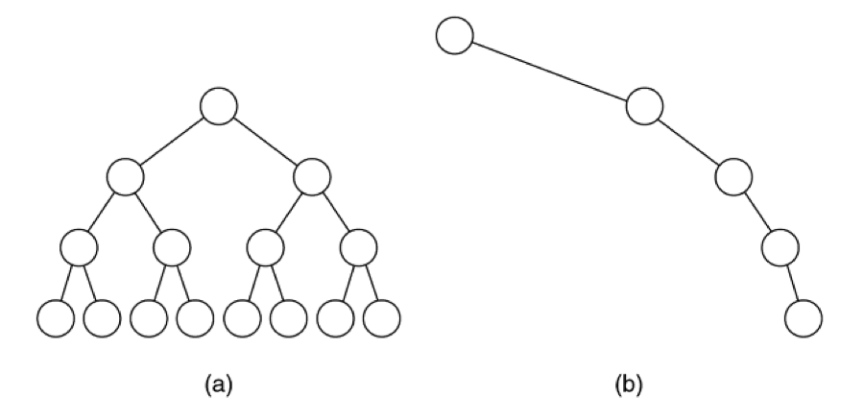
\includegraphics[width=0.5\textwidth,height=\textheight]{images/1.png}
\caption{(a) The balanced tree has a depth of
\(\lfloor \log(n) \rfloor\); (b) the unbalanced tree has a depth of
\(n-1\)}
\end{figure}

\hypertarget{balancing-trees}{%
\subsection{Balancing Trees}\label{balancing-trees}}

\begin{itemize}
\tightlist
\item
  Self-balancing binary search trees

  \begin{itemize}
  \tightlist
  \item
    Prevent degenerated trees by keeping the tree balanced
  \item
    Need re-balancing on \passthrough{\lstinline!insert(T t)!} or
    \passthrough{\lstinline!remove(T t)!}
  \item
    Need to maintain additional properties beyond being a search tree
  \end{itemize}
\item
  Several kinds of trees do this

  \begin{itemize}
  \tightlist
  \item
    AVL: the left and right subtree height differs by no more than \(1\)
  \item
    Red-black: preserve \(4\) red/black node properties
  \item
    B-trees: the generalized version with \(m\) children (we'll revisit
    this later in the semester)
  \item
    AA: a red-black tree where all the left nodes are black
  \item
    Splay: a tree where recently accessed elements are faster accessed
    than less recently accessed elements
  \end{itemize}
\end{itemize}

\hypertarget{avl-trees}{%
\subsection{AVL Trees}\label{avl-trees}}

\begin{itemize}
\tightlist
\item
  The AVL tree is named after its two inventors, Georgy Adelson-Velsky
  and E.M. Landis, who published it in their 1962 paper \enquote{An
  algorithm for the organization of information}
\item
  Definition: an AVL tree is a balanced binary search tree. For any
  \passthrough{\lstinline!Node n!} in an AVL tree:

  \begin{itemize}
  \tightlist
  \item
    \passthrough{\lstinline!n.left!} and
    \passthrough{\lstinline!n.right!} differe in height by at most
    \passthrough{\lstinline!1!}
  \item
    The leaf node has a height \passthrough{\lstinline!0!}
  \item
    \passthrough{\lstinline!null!} (the empty subtree) has a height of
    \passthrough{\lstinline!-1!}
  \end{itemize}
\item
  AVL tree is a self-balancing tree

  \begin{itemize}
  \tightlist
  \item
    Make adjustments at insertion/removal to keep the tree balanced
  \end{itemize}
\end{itemize}

\hypertarget{exercise-spot-the-avl-trees}{%
\subsection{Exercise: Spot the AVL
Trees}\label{exercise-spot-the-avl-trees}}

\begin{figure}
\centering
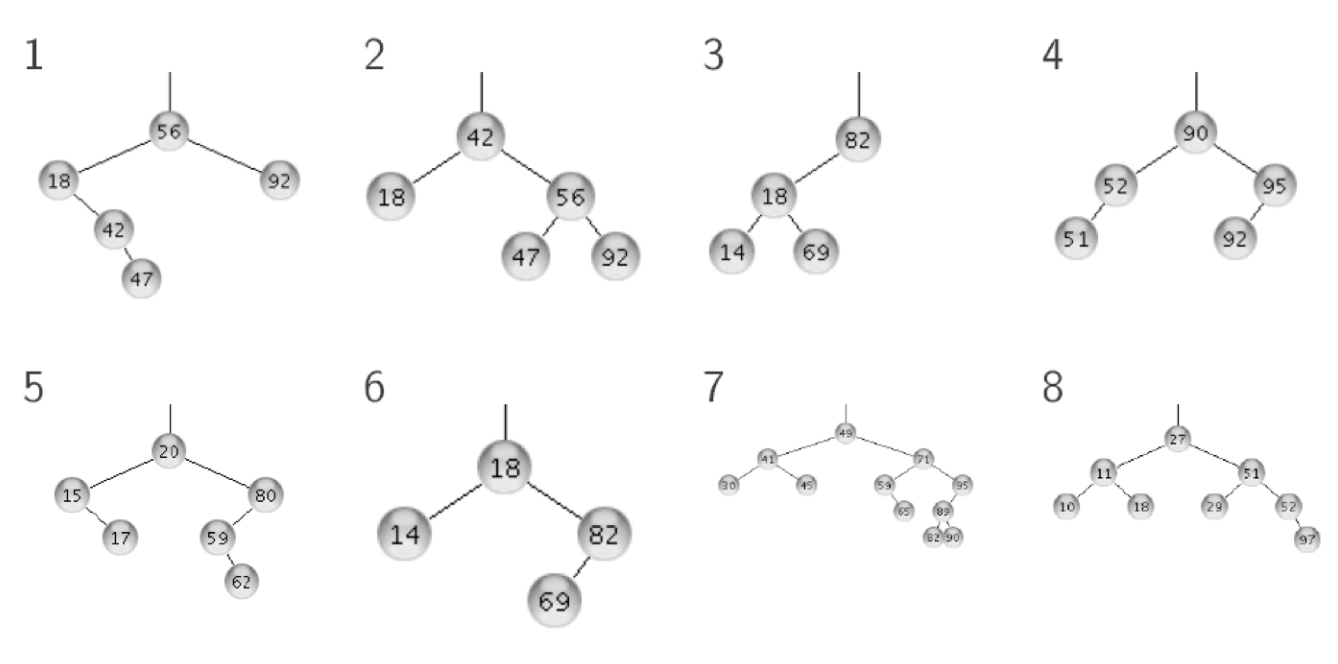
\includegraphics[width=0.75\textwidth,height=\textheight]{images/2.png}
\caption{Can you spot the Possible AVL Trees}
\end{figure}

\begin{itemize}
\tightlist
\item
  \textbf{TODO: LIST THE AVL TREES}
\end{itemize}

\hypertarget{avl-trees-balancing}{%
\subsection{AVL Trees: Balancing}\label{avl-trees-balancing}}

\begin{itemize}
\tightlist
\item
  Track the balance factor of tree nodes

  \begin{itemize}
  \tightlist
  \item
    \passthrough{\lstinline!balance = height(n.left) - height(n.right)!}
  \item
    Must be \passthrough{\lstinline!-1!}, \passthrough{\lstinline!0!},
    or \passthrough{\lstinline!+1!} for it to be an AVL tree

    \begin{itemize}
    \tightlist
    \item
      If it is any other value, we must perform rotations in the tree
    \end{itemize}
  \end{itemize}
\item
  Key idea: track and adjust the balance on
  \passthrough{\lstinline!insert(T t)!} or
  \passthrough{\lstinline!delete(T t)!}

  \begin{itemize}
  \tightlist
  \item
    Recursively add or remove a node
  \item
    Unwind the recursion up to adjust the balance of the ancestors

    \begin{itemize}
    \tightlist
    \item
      Observation: only nodes along the path from changing point to root
      may need to (potentially) be balanced
    \end{itemize}
  \item
    When unbalanced, rotate to adjust heights

    \begin{itemize}
    \tightlist
    \item
      Rotation changes structure of tree without affecting ordering
    \item
      Might need single or double rotation
    \end{itemize}
  \end{itemize}
\end{itemize}

\hypertarget{avl-tree-insertion}{%
\subsection{AVL Tree Insertion}\label{avl-tree-insertion}}

\begin{itemize}
\tightlist
\item
  Start the same as a normal binary search tree insertion
\item
  When a node is added too deep, the balance is broken

  \begin{itemize}
  \tightlist
  \item
    We need to fix the broken cases with rotation
  \end{itemize}
\end{itemize}

\hypertarget{single-rotations-basics}{%
\subsection{Single Rotations Basics}\label{single-rotations-basics}}

\begin{itemize}
\tightlist
\item
  Right rotation

  \begin{itemize}
  \tightlist
  \item
    The left child becomes the new root, and the old root becomes the
    right child
  \end{itemize}
\end{itemize}

\begin{figure}
\centering
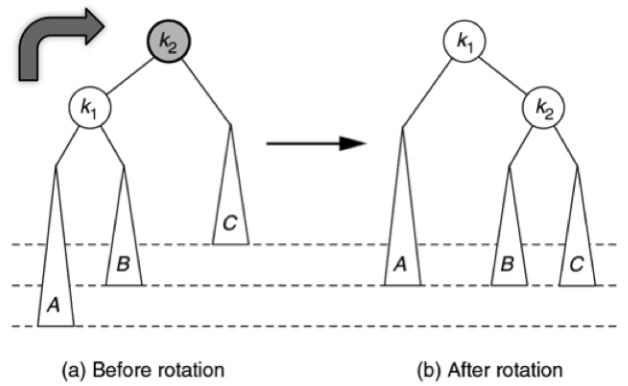
\includegraphics[width=0.5\textwidth,height=\textheight]{images/3.png}
\caption{AVL tree under right rotation}
\end{figure}

\begin{itemize}
\tightlist
\item
  Left rotation

  \begin{itemize}
  \tightlist
  \item
    The right child becomes the new root, and the old root becomes the
    left child
  \end{itemize}
\end{itemize}

\begin{figure}
\centering
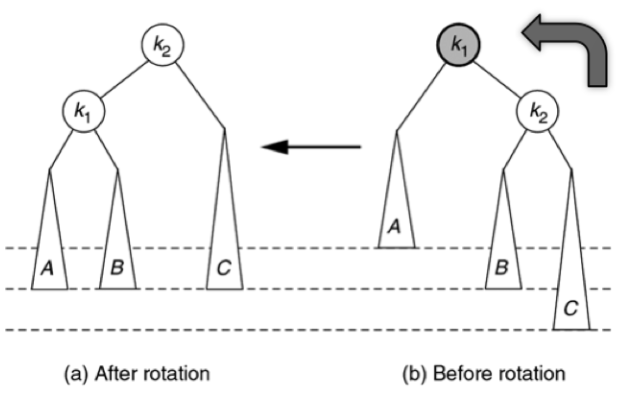
\includegraphics[width=0.5\textwidth,height=\textheight]{images/4.png}
\caption{AVL tree under left rotation}
\end{figure}

\hypertarget{single-rotation-to-fix}{%
\subsection{Single Rotation to Fix}\label{single-rotation-to-fix}}

\begin{figure}
\centering
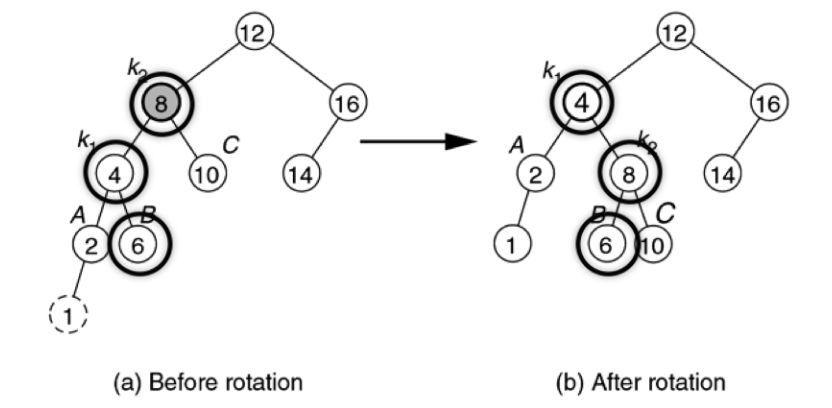
\includegraphics[width=0.5\textwidth,height=\textheight]{images/5.png}
\caption{Single rotation fixes an AVL tree after insertion of 1}
\end{figure}

\hypertarget{re-balancing-with-a-single-rotation}{%
\subsection{Re-Balancing with a Single
Rotation}\label{re-balancing-with-a-single-rotation}}

\begin{figure}
\centering
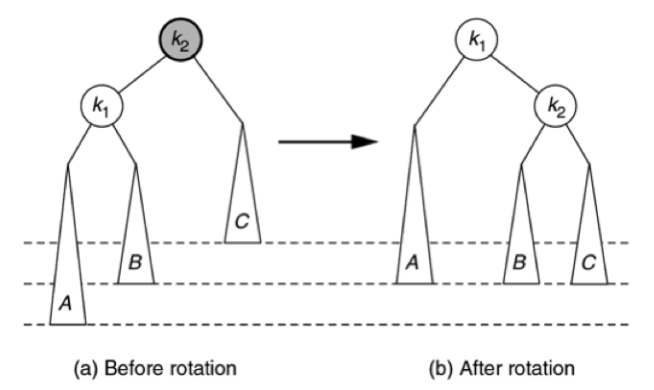
\includegraphics[width=0.5\textwidth,height=\textheight]{images/6.png}
\caption{Single Rotation}
\end{figure}

\begin{itemize}
\tightlist
\item
  Why does this work?

  \begin{itemize}
  \tightlist
  \item
    \{node in A\} \(< k_1 <\) \{node in B\} \(< k_2 <\) \{node in C\}
  \item
    The height difference is reduced
  \end{itemize}
\end{itemize}

\begin{lstlisting}[language=Java]
// Single Right rotation
Node<T> rightRotate(Node<T> t) { // t is the old root, k_2
  Node<T> newRoot = t.left; // promote k_1
  t.left = newRoot.right;   // k_2 takes over B as the left child
  newRoot.right = t;        // k_1 takes over k_2 as the right child
  t.height = Math.max(t.left.height, t.right.height) + 1; // update the height
  newRoot.height = Math.max(newRoot.left.height, newRoot.right.height) + 1;
  return newRoot;
}
\end{lstlisting}

\hypertarget{practice}{%
\subsection{Practice}\label{practice}}

\hypertarget{example-1}{%
\subsubsection{Example 1}\label{example-1}}

\begin{itemize}
\tightlist
\item
  Insert 40
\item
  Which node(s) need(s) to be re-balanced?
\item
  How do we re-balance it?
\end{itemize}

\begin{figure}
\centering
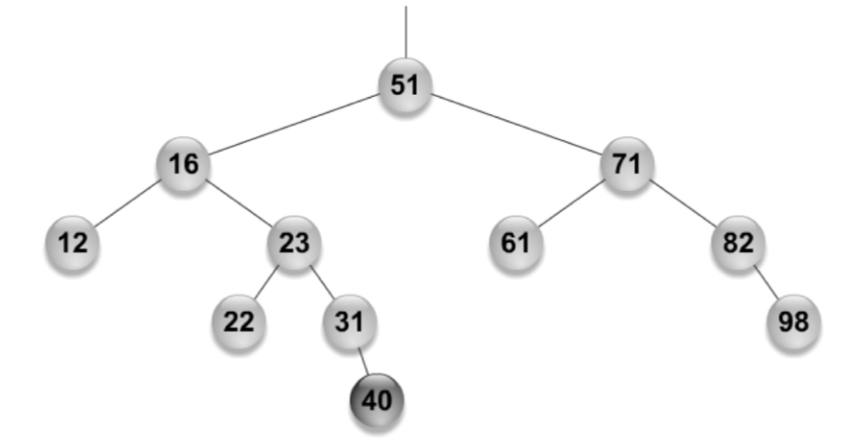
\includegraphics[width=0.5\textwidth,height=\textheight]{images/7.png}
\caption{Example 1}
\end{figure}

\hypertarget{example-2}{%
\subsubsection{Example 2}\label{example-2}}

\begin{itemize}
\tightlist
\item
  Insert 85
\item
  Which node(s) need(s) to be re-balanced?
\item
  How do we re-balance it?
\end{itemize}

\begin{figure}
\centering
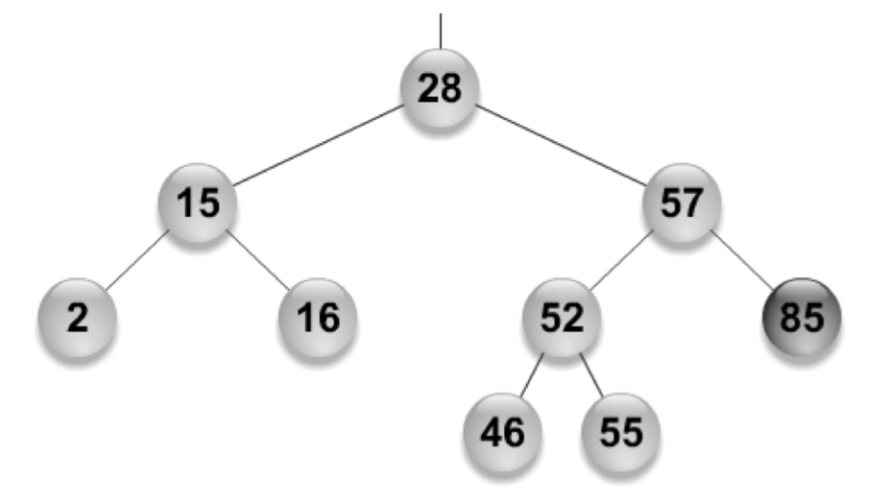
\includegraphics[width=0.5\textwidth,height=\textheight]{images/8.png}
\caption{Example 2}
\end{figure}

\hypertarget{multiple-rotation-basics}{%
\subsection{Multiple Rotation Basics}\label{multiple-rotation-basics}}

\begin{itemize}
\tightlist
\item
  Sometimes a single insertion isn't enough
\end{itemize}

\begin{figure}
\centering
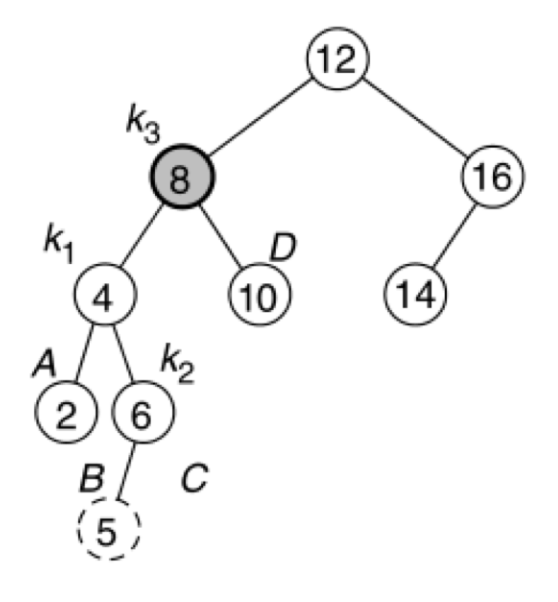
\includegraphics[width=0.25\textwidth,height=\textheight]{images/9.png}
\caption{AVL tree with insertion that necessitates multiple rotations}
\end{figure}

\begin{itemize}
\tightlist
\item
  Here we insert 5
\item
  The AVL tree is now unbalanced -- how do we fix it?

  \begin{itemize}
  \tightlist
  \item
    Rotation like before doesn't work:
  \end{itemize}
\end{itemize}

\begin{figure}
\centering
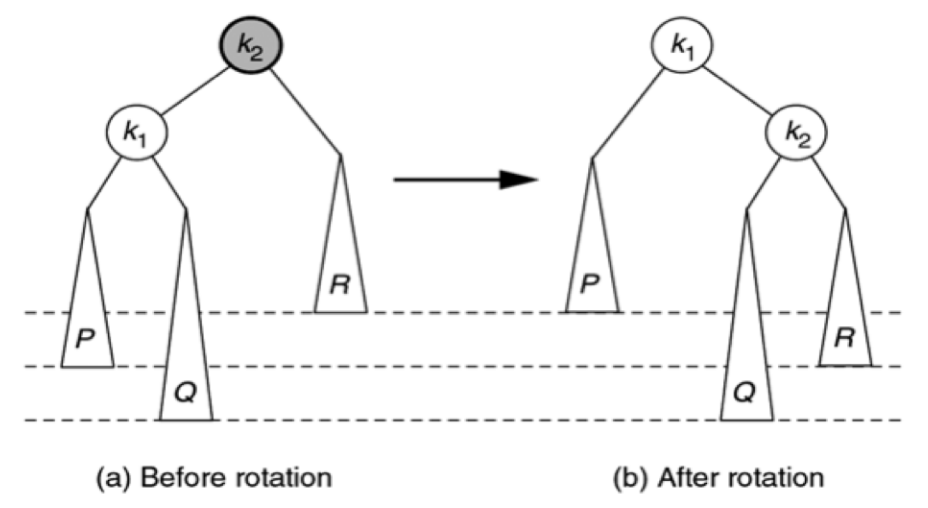
\includegraphics[width=0.5\textwidth,height=\textheight]{images/10.png}
\caption{AVL tree which remains broken under single rotations}
\end{figure}

\begin{itemize}
\tightlist
\item
  The tree keeps the same height difference that it had before the
  rotation
\item
  How can we fix this?

  \begin{itemize}
  \tightlist
  \item
    With double rotations!
  \end{itemize}
\end{itemize}

\hypertarget{left-right-double-rotation}{%
\subsection{Left-Right Double
Rotation}\label{left-right-double-rotation}}

\begin{itemize}
\tightlist
\item
  Left rotate \((k_1, k_2)\)
\item
  Right rotate \((k_3, k_2)\)
\end{itemize}

\begin{figure}
\centering
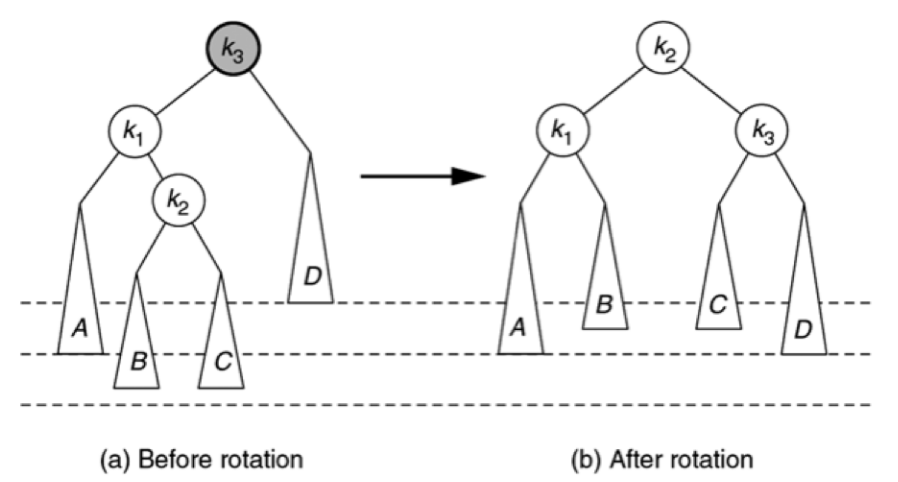
\includegraphics[width=0.5\textwidth,height=\textheight]{images/11.png}
\caption{AVL tree with double rotation}
\end{figure}

\hypertarget{double-rotation-example}{%
\subsection{Double Rotation Example}\label{double-rotation-example}}

\begin{itemize}
\tightlist
\item
  Insert 5

  \begin{itemize}
  \tightlist
  \item
    The problem is at 8: the left and right heights differ by 2

    \begin{itemize}
    \tightlist
    \item
      Left rotate 4 (the height imbalance remains)
    \item
      Right rotate 8 (the height imbalance is fixed)
    \end{itemize}
  \end{itemize}
\end{itemize}

\begin{figure}
\centering
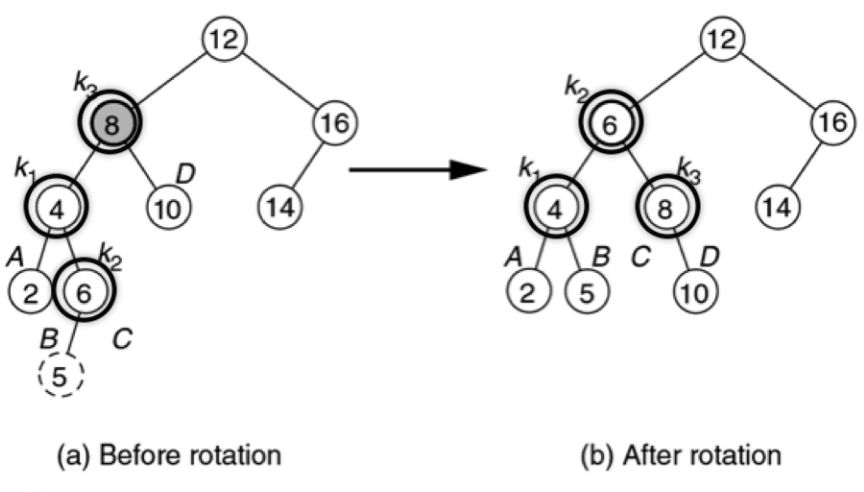
\includegraphics[width=0.5\textwidth,height=\textheight]{images/12.png}
\caption{An example AVL tree with double rotation}
\end{figure}

\end{document}
